\documentclass{exos}
\usepackage{main}

\title{Activité : Représentation graphique de fonctions}
\author{Seconde 3}
\date{19 Novembre 2025}

\begin{document}
\maketitle

\section{Repère orthonormé}
\begin{center}
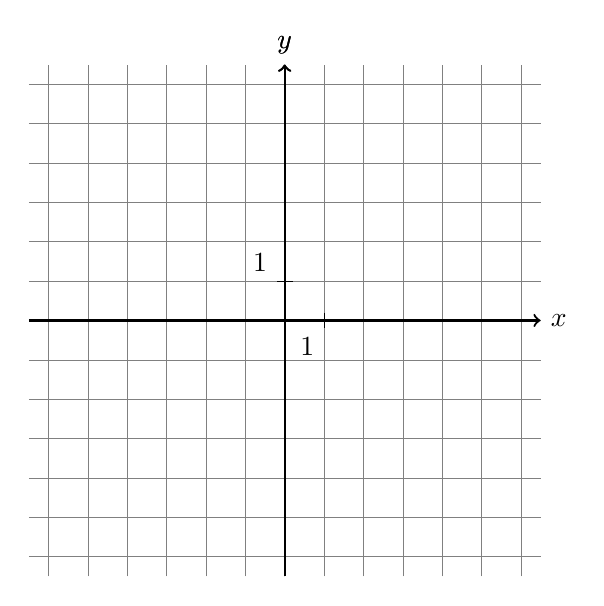
\begin{tikzpicture}
\draw[help lines] (-3.25,-3.25) grid[step=0.5] (3.25,3.25);
\draw[thick,->] (-3.25,0) -- (3.25,0) node[right] {$x$};
\draw[thick,->] (0,-3.25) -- (0,3.25) node[above] {$y$};
\draw[thick,->] (0,-3.25) -- (0,3.25) node[above] {$y$};
\draw (0.5,0.1) -- (0.5,-0.1) node[below left] {$1$};
\draw (0.1,0.5) -- (-0.1,0.5) node[above left] {$1$};
\end{tikzpicture}
\end{center}

\begin{alphaquestions}
\begin{minipage}{0.4\textwidth}
  
  \item Choisissez deux nombres $x$ et $y$. Placer un point $A$ dont les coordonnées correspondent aux deux nombres.
  \item Choisissez un nombre $b$. Placer un point $B$ dont l'abscisse est $b$ et dont l'ordonnée est le double de $b$.
  \item Recommencer la question précédente pour placer trois autres points $C$; $D$; $E$ dont l'ordonnée est le double des abscisse.
  \item Placer au moins mille point vérifiant cette relation entre abscisse et ordonnée. (Indication : un trait continu est constitué d'une infinité de points)
  
  \begin{tcolorbox}
    La courbe que vous avez dessinée est appelée \textbf{courbe représentative de la fonction $f : x \mapsto 2 \times x$}
  \end{tcolorbox}
\end{minipage}
\hfill\vline\hfill
\begin{minipage}{0.4\textwidth}  
\item Donner une relation entre les abscisses $x$ et les ordonnées $y$ des points la courbe que vous avez tracé à l'aide de $f$.

\item Soit $g : x \mapsto -x$. Placer plusieurs point de la courbe représentative de $g$ sur le repère. En déduire un tracé de la courbe représentative de $g$.

\item (Pour aller plus loin) Tracer sur un repère orthonormé une courbe qui n'est \textsc{PAS} la courbe représentative d'une fonction.
\end{minipage}
\end{alphaquestions}
\end{document}